% One summand of the three-block chain rule in (F18)--(F21).
% The coordinate nodes and arrows adapt expert_column.tex's address diagram.
\documentclass[tikz,border=0pt]{standalone}
\usepackage{amsmath}
\usetikzlibrary{arrows.meta,backgrounds,positioning}
\definecolor{addr}{RGB}{40,90,150}
\begin{document}
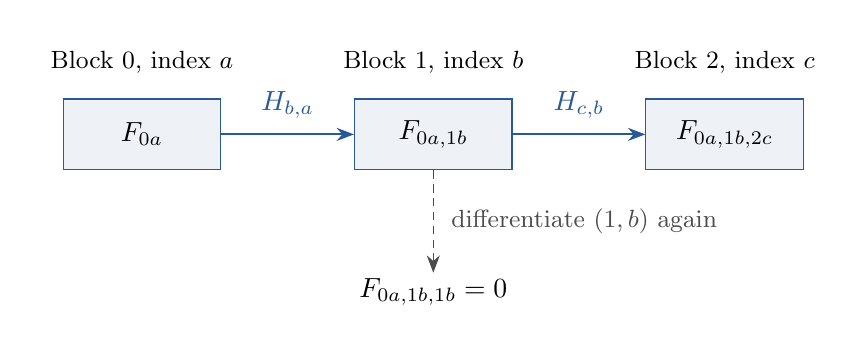
\begin{tikzpicture}[
  font=\normalsize,
  show background rectangle, background rectangle/.style={fill=white},
  inner frame sep=5pt,
  >={Stealth[length=2.2mm]},
  coordinate derivative/.style={draw=addr, fill=addr!8,
    minimum width=20mm, minimum height=9mm, inner xsep=5pt},
  crossing/.style={->, addr, thick},
  block/.style={above=2mm, font=\small}]
\node[coordinate derivative] (a) at (0,0) {$F_{0a}$};
\node[coordinate derivative] (b) at (3.7,0) {$F_{0a,1b}$};
\node[coordinate derivative] (c) at (7.4,0) {$F_{0a,1b,2c}$};
\node[block] at (a.north) {Block $0$, index $a$};
\node[block] at (b.north) {Block $1$, index $b$};
\node[block] at (c.north) {Block $2$, index $c$};
\draw[crossing] (a.east) -- node[above=2pt] {$H_{b,a}$} (b.west);
\draw[crossing] (b.east) -- node[above=2pt] {$H_{c,b}$} (c.west);
% In (F20), entering the middle bias through U'_b can only repeat (1,b).
\node[below=13mm of b, inner sep=2pt] (repeat) {$F_{0a,1b,1b}=0$};
\draw[->, densely dashed, black!70] (b.south) --
  node[right=3pt, font=\small] {differentiate $(1,b)$ again} (repeat.north);
\end{tikzpicture}
\end{document}
